% 来源：OEBPS/Text/Section0001_split_005.xhtml#sigil_toc_id_36

\BookChapter{25}
\section[第25章\q 选时重于一切]{第25章\\ 选时重于一切}

\begin{BookQuote}
我们遇见敌人了，敌人就是我们自己。

\hfill ——波戈
\end{BookQuote}

对于投资者和单人脱口秀演员来说，共同的成功秘诀是什么？

选时。选时决定一切。

最好的喜剧演员知道什么时候抖包袱才恰到好处。最聪明的投资者知道，什么时候进入市场才恰到好处，但他们不知道是否应该进入市场。即使投资大师也不可能每一次都正好踩到点上。对于一个喜剧演员来说，时机没把握好，整个剧场的气氛会十分尴尬，死一般的沉默——也许还有观众大骂着往台上扔东西。如果你是个投资者，选择时机出现错误可能会毁掉你一辈子积攒的养老金。所以，我们需要找到一个解决方法，它并不需要我们成为一个通灵大师，上知天意，下知地意，上知500年，下知500年。

我们已经知道，如何把自己的投资组合分散到不同资产类型的市场，以在波动无常的经济中保护自己的资产价值稳定增长。但是，我们所有人都有过这样的经历，既出现在了正确的地方，又做出了完全正确的事，可是我们把时机选错了。所以现在你可能会想：“好了，托尼，现在我知道如何分散我的投资了，但是如果我的时机选择错误了呢？”

我也问过自己同样的问题：万一我把钱投入股市正好是在最高点，买入之后股市就开始下跌，我怎么办？或者我买了一只债券基金，然后利率开始大幅提高，结果我的债券基金开始暴跌，我又该怎么办？市场总会波动，我们已经知道了，没有一个人，我的意思是说绝对没有一个人，能够持续地成功预测未来。

所以我们如何保护自己，避免受到这些市场起伏、涨跌的冲击，真正取得成功？

大多数投资者都陷入了一种盲从的心态，他们追逐赢家，远离输家，在股市上追涨杀跌。公募基金经理也会做同样的事。这是人类的天性，想要追随大众，不愿意错过任何好事。“情绪控制着我们人类，我们投资者也是人，容易做出非常愚蠢的事。”普林斯顿大学经济学家伯顿·麦基尔告诉我，“我们想要选择正确的时机，低买高卖，低位进入市场，高位卖出，但实际上我们往往选择了错误的时机，高买低卖，该买的时候卖了，该卖的时候买了。”

\begin{figure}[htbp]
\centering
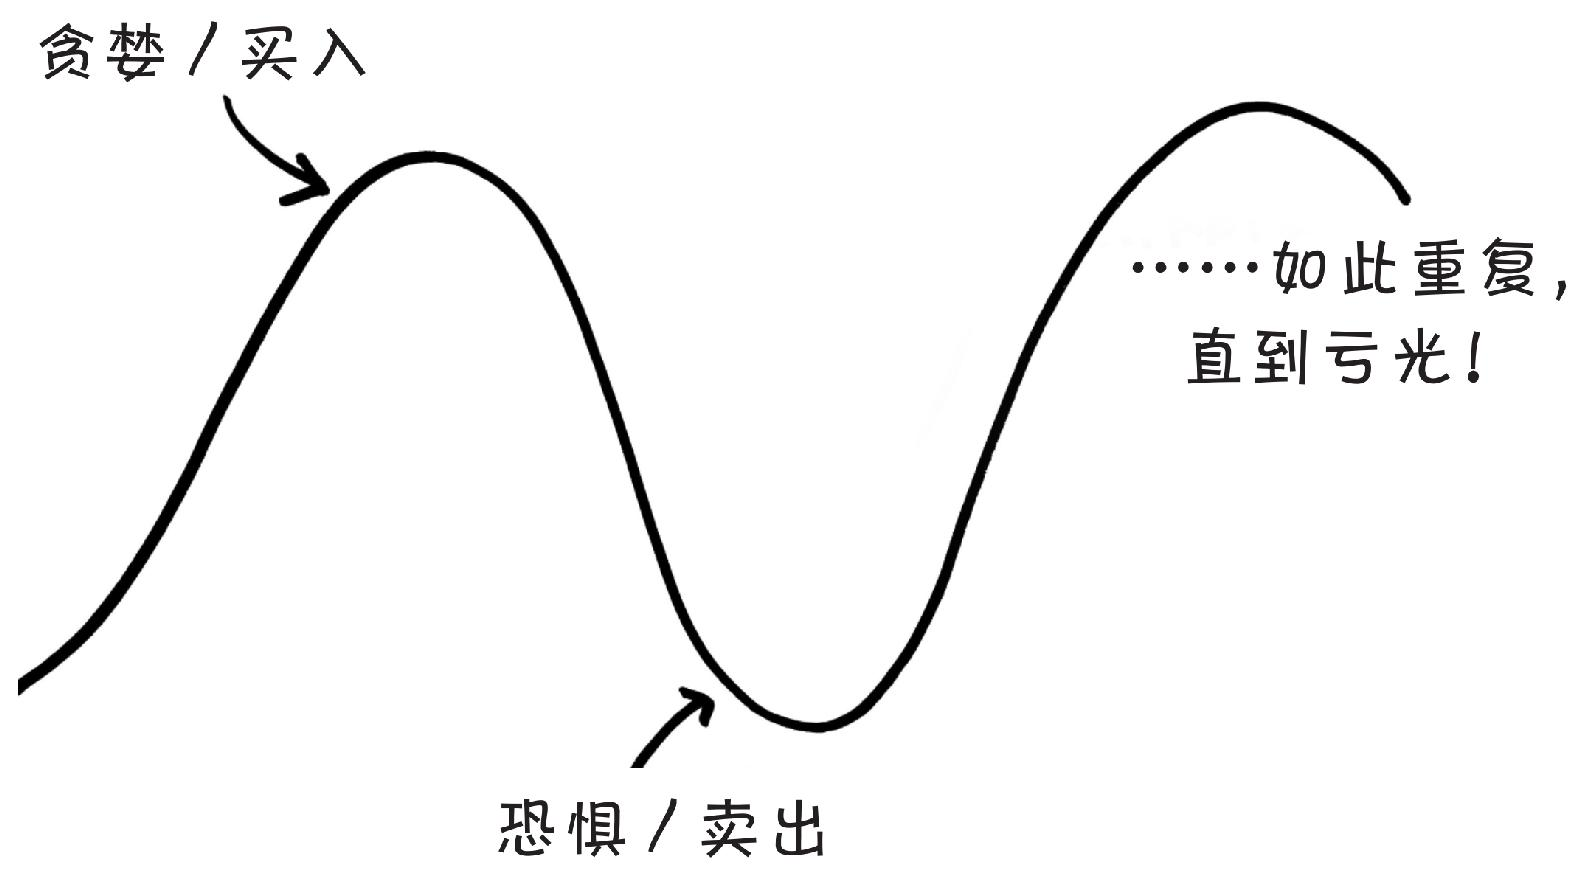
\includegraphics[width=0.72\linewidth,keepaspectratio]{image/25-1.jpg}
\caption{}\label{fig:25-1}
\end{figure}

他提醒我关注一下21世纪初科技泡沫期间发生的事情：“2000年第一季度，更多的资金进入股市，这个时候正好是股市网络股泡沫的顶点，股市从来没有涨到过这么高。”他说，“后来到了2002年第三季度，市场一路下跌，资金大量出逃。”那些经受不住大跌考验而迅速逃跑的投资者，结果错过了十年来最大一波反弹。“然后到2008年第三季度，正好金融危机也同时达到了顶点。”麦基尔说，“更多的资金退出股市，资金规模比以前任何时期都大。结果后来又出现了一波更大的反弹。所以，我们的情绪掌控了我们。我们被吓坏了。”

股市出现前所未见的暴跌，我们被吓坏了，赶紧卖出逃跑，这很正常。谁又能责怪谁呢？2009年10月，美国股市市值蒸发了2万亿美元，每个月都有几十万名美国人失业，这时美国全国广播公司的《今日秀》节目主持人马特·劳尔打电话到我的办公室。他让我第二天早晨参加他的节目，谈谈美国人应该如何应对这场危机。我认识马特好多年了，我也参加过好几次他的节目，所以我马上就同意了。我一到演播室，节目制片人就告诉我：“你来了就好了，你有4分钟的时间给整个美国打打气。”

我心里想：“你开玩笑吧？”

“给大家打气并不是我要做的。”我说，“我要告诉他们真相。”这正是我那天所做的事情。在《今日秀》节目两个不同的时段，我警告观众，股市崩盘还没有结束，最坏的情况可能正在逼近。我怎么能给观众打气呢？

“现在很多股票的价格暴跌，不久之前还卖50美元的股票，现在只卖10美元，甚至只有5美元。这里我要告诉你的真相是：有些股票可能还会跌到1美元。”我这样一说，新闻主持人马特·劳尔的眼睛瞪得越来越大。但是我也告诉观众，与其让暴跌吓呆了，完全崩溃，不如跟自己的恐惧做斗争，好好教育自己，多学学那些在股市崩溃时期做得很好的投资大师。就像约翰·邓普顿爵士，他在20世纪30年代美国经济大萧条时期，在股市暴跌的时候却赚够了钱。我说，如果你研究历史，就会知道股市暴跌之后会有一次大反弹，这是让你赚大钱的机会，根据20世纪70年代，甚至是30年代发生的事情，在短期之内那些从50美元暴跌到1美元的股票会再次反弹，它们也许再也不会反弹到50美元，但是很多股票会在几个月之内反弹到5美元，这意味着400\%的收益率，而且是发生在6个月之内！“所以如果你保持内心强大，头脑聪明，随着股市持续反弹，你可能会赚到10倍甚至更高的收益！这可能是你有生以来最伟大的投资机会！”我说。

这并不完全是《今日秀》节目希望我能让观众们知道的东西，但是结果证明我说的完全正确。我怎么知道市场还会继续下跌？是不是因为我太聪明了？根本不是。真相是，我的朋友保罗·都铎·琼斯一直在警告我市场会发生什么情况，他早在这场危机发生一年之前就警告过我了。能够持续预测市场走势的人凤毛麟角，而他绝对是其中之一。其中一部分原因让他不仅成为有史以来最成功的投资者，而且是一个传奇性人物。他预测出1987年美国股市黑色星期一的大崩盘，在其他所有人都吓得四散而逃的时候，他却帮助他的客户一个月赚了60\%，一年赚了200\%。

所以，我非常感激保罗能够洞察股市先机。2008年年初，他告诉我，股市和楼市双双大崩盘就要来了，而且很快就要来了。我一听非常重视，马上去找我的白金合伙人。白金合伙人是由我的一些高端客户组成的封闭性小群体，我一年和他们有三四次聚会，小规模密集地沟通和指导他们，以增进他们的夫妻关系，以及改善企业经营和投资理财。我召集了一个紧急会议，让他们都飞过来和我见面，地点在迪拜，时间是在2008年4月。在会上，我警告他们即将到来一场危机，以帮助他们做好准备。记住，预测就是力量。由于提前3\textasciitilde{}6个月跳出了股市和楼市，我的很多客户实实在在地赚到了钱，因为后来发生了有史以来最大的经济危机。

是的，完全可以确定的是，股票价格在2008年第四季度一直暴跌。到了2009年3月，股市行情简直太糟糕了，花旗银行的股价从最高峰的每股57美元跌到，你能猜到吗，正如我警告过的那样，真的跌破了1美元，跌到了0.97美元。你买这只股票所花的钱，比你从这家银行自动取款机里取一次钱要交的手续费还要少。

那么在这种极端情形下，投资者应该怎么办？如果你相信约翰·邓普顿爵士的名言“好的机会来自悲观情绪最严重的时候”，或者巴菲特的投资魔咒“在别人都贪婪的时候恐惧，在别人都恐惧的时候贪婪”，那么现在正是一个大量抢购便宜货的绝佳时机。为什么？因为聪明的长期投资者都知道，季节总是在变的。他们会告诉你，冬天才是买入的好时机——2009年年初的几个月，绝对可以说是投资的冬天！这是赚大钱发大财的时候，因为尽管需要等上一段时间，但是春天总是会来的。

但是如果你被吓坏了，或者觉得必须卖出股票，因为整个股市都崩溃了，那么结果会怎么样？你也许会说：“托尼，如果我2008年丢了工作，而且没有其他收入来源，我该怎么办？或者我的孩子要交学费了，银行一分钱也不肯贷给我，除了卖股票，我还能怎么办？”如果你在2008年暴跌之中卖掉了股票，我只能说我能感受到你的痛苦，但我希望你能够找到别的办法弄到钱，以满足这些家庭生活的基本开支。个人投资者在市场暴跌之后清仓，卖出了手上的基金或股票，他们都从中学到了痛苦的教训。他们并没有趁着股市大反弹而重新杀回来。他们亏怕了，再也不敢进股市了，就这样他们锁定了自己的损失——永远。如果他们再重新回到股市，那时候他们必定要支付高得多的价格，因为你知道那时肯定是股市大幅快速上涨，恢复生机的时候。

看到这么多人在这么短的时间亏掉了这么多钱，并由此引发巨大的痛苦，这让我非常痛苦。于是，我开始执着地想做一件事：把最重要的投资智慧带给众多普通投资者。正是这一点促成了本书的诞生。

这让我想弄明白同样的金融科技工具能创造出高频交易（高频交易者真的只有上行收益而没有下行风险），是不是可以用某种方式利用这种高科技，让一般投资者也能从中得到好处？记住，高频交易投资者总能赚钱，他们几乎从来不亏钱。

那么好消息是什么？接下来你会学到一个办法，可以让你从来不会离开市场，也不会承受一点儿损失。为什么？因为有金融工具，具体来说是保险产品，你根本不用担心如何选择进出市场的时机。市场上涨，你就会跟着赚钱，市场下跌10\%、20\%、30\%，甚至50\%的时候，你也一分钱不会亏（按照保险公司的保证条款）。这听起来简直太好了，好像不可能是真的，但是这确实是真实的。这种终极金融工具能给你创造一种赚钱的投资组合，让你感到内心的真正安宁。现在让我们来看看这种工具，它能够帮助你限制大多数的投资风险，同时使投资收益率增加到最高的水平，而它借助的却是一种很传统的投资模式。

\begin{BookQuote}
未来不会和过去一样。

\hfill ——约吉·贝拉
\end{BookQuote}

\begin{BookQuote}
预测是非常困难的，特别是预测未来。

\hfill ——尼尔斯·波尔
\end{BookQuote}

2009年3月2日，保罗·都铎·琼斯告诉我，市场就要跌到绝对底线了。股价反弹，股市又开始上涨了。股市的春天要来了，于是我发了几条推特：

市场从来不会有错。舆论才会经常出错。声名狼藉的交易员杰西·利弗莫尔说：“我并不是一个选时的人。祝你好运。托尼。”

教育你自己，做出你自己的独立决策。只做你能承担得起损失的交易……我并不是要教育人，只是赞成一定要小心谨慎。

我给世界顶级的交易员做人生教练（到现在有17年了）。我不是给他们关于交易的建议，而是常常提醒他们要关注可能的底部正在来临。

顺便说一下，这是我第一次发推特谈论关于股票市场的未来走势！结果是只过了7天，美国股票交易所指数的走势完全和我预测的一模一样：3月9日触底反弹。股价开始是缓慢上涨，后来是快速上涨。可以肯定的是，花旗银行的股票，2009年3月9日的收盘价为1.05美元，2009年8月27日的收盘价为5美元——不到5个月上涨了400\%！\footnote{\label{fn:pdf-25-1}看看今天大多数财经网站或者软件提供的股票行情走势图，你会看到花旗银行的股票行情的历史价格：2009年3月9日收盘价为10.50美元，2009年8月27日收盘价为50.50美元。但这些价格并不准确。这些图表没有进行复权处理，来反映2011年5月6日花旗银行做的反向股票分割（10股合并成1股）。5月5日股价还是每股4.48美元的股票，第二天5月6日每10股合并成1股，就成了每股44.80美元，当日收盘价是每股45.20美元，小幅上涨0.4美元，接近1\%。原来花旗银行的股票总共有290亿股，10股合并成1股之后，股票总数只有29亿股，它的目的只有一个，就是抬高每股股价。正如《华尔街日报》在2011年5月10日所说的那样：“从2007年以来花旗银行首次成为一只股价达到40美元的股票，按照星期五的收盘价，股价看起来涨幅超过850\%。警告，投资者一分钱也没挣到。”}不到半年能够赚到这么高的收益率简直令人不可思议，前提是你能够管住自己内心的恐惧，在别人都在卖出的时候大胆买入，你才能赚到钱！

现在我真希望，过去市场行情可以预测未来的市场走势。保罗·都铎·琼斯或者其他我知道的人，能够持续成功地预测这些市场的大起大落。但是这是不可能的。基于那些“股市消息灵通人士”的分析，我在电视上又一次提前发出警告，2010年股市可能再次出现一波大跌，当时股市似乎涨得过头了，面临一波大跌来修正，我希望人们清醒地做出决策，保护自己，避免遭受可能出现的另一次重大打击。但是这次我错了。没有人预测到美国政府出手救市的手段这么狠，人类历史上从来没有一个国家的政府敢这么干——美国政府决定推动市场上涨，手段是“印”4万亿美元的钞票，同时告诉全世界，美国政府会持续这么做下去，无限地持续做下去，直到经济复苏为止。

就这样，政府资产负债表上的资产增加了好多个零，美联储能够把现金注入经济体系，办法是从大型银行手里回购债券（包括住房抵押债券和国债），银行把债券给美联储，美联储把自己印的钞票给银行，银行再把这些钞票贷出去，就这样，政府把货币注入了经济体系。发行的货币太多了，利率就降到了非常低的水平，美联储由此就能持续保持利率在极低的水平，低到接近于零。那些原来存款的人和原来买债券的人拿到手的固定收益率简直太低了，这相当于逼着他们进入股市去寻找还过得去的较高收益率。美联储年复一年地持续这样操作。所以一点儿也不奇怪，在这样巨大的资金推动下，美国股票从来没有下跌过。

\begin{figure}[htbp]
\centering
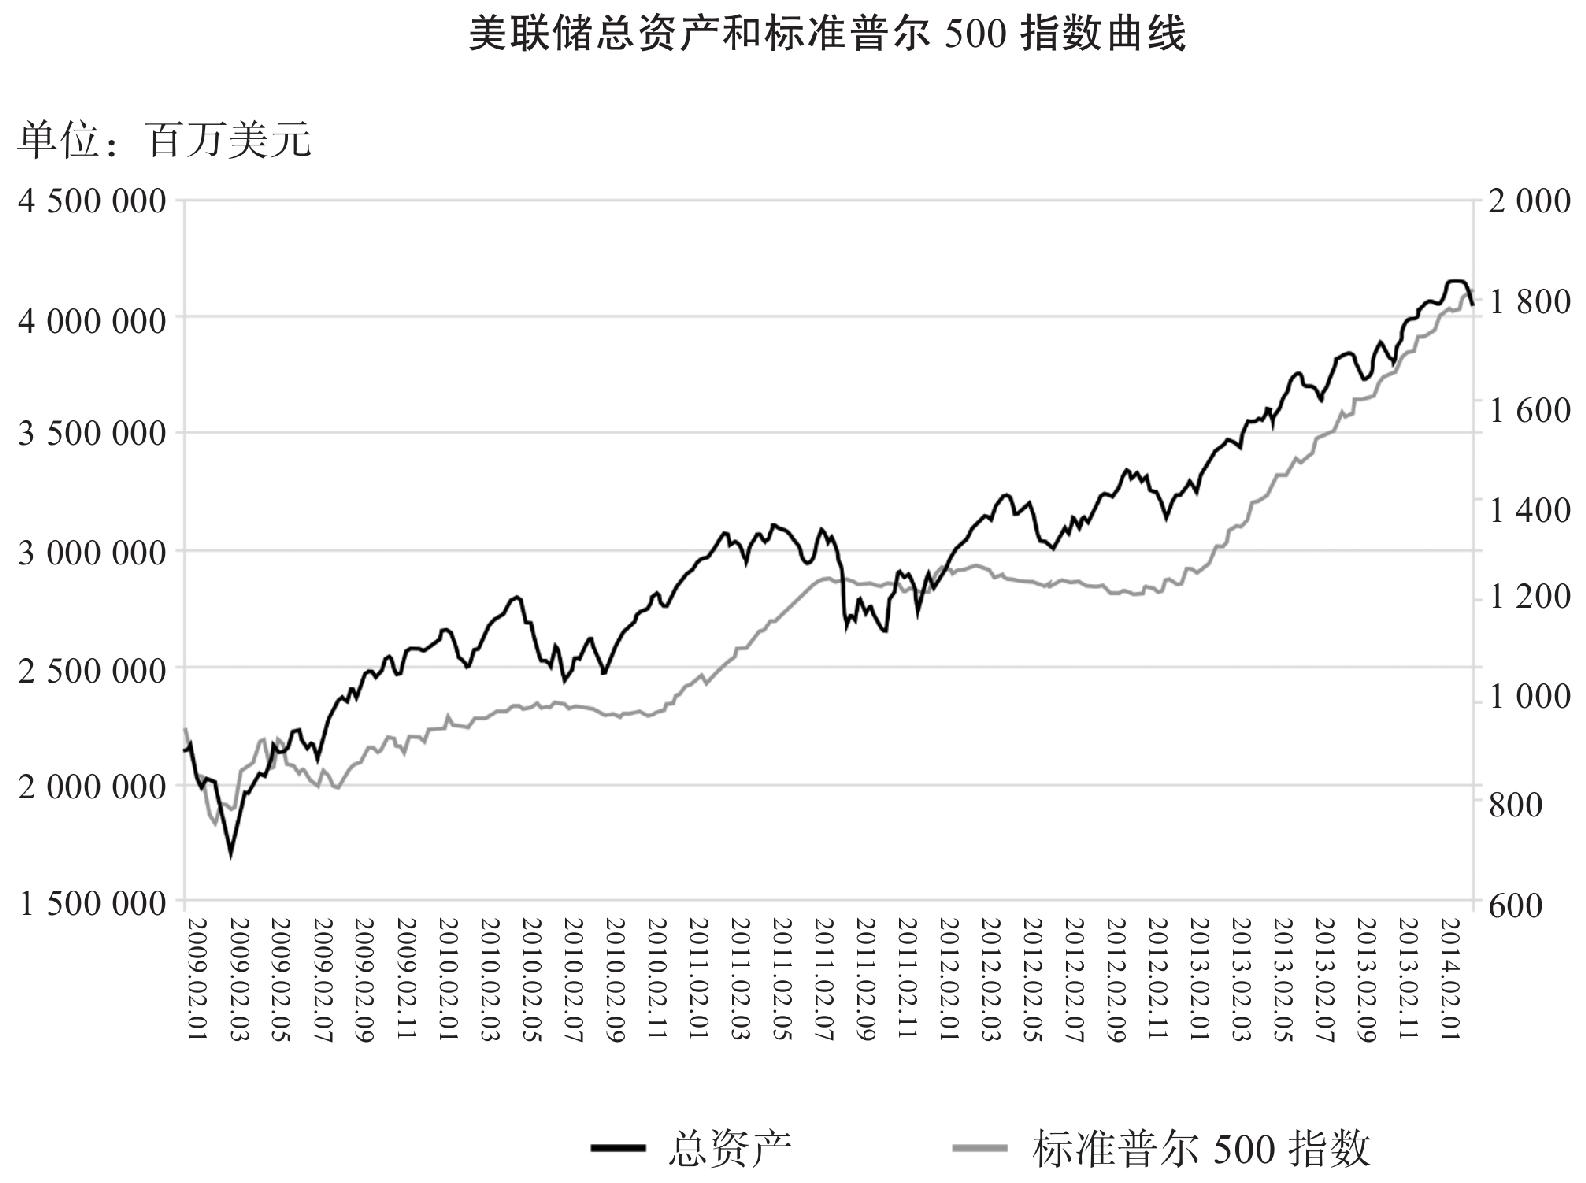
\includegraphics[width=0.96\linewidth,keepaspectratio]{image/25-2.jpg}
\caption{}\label{fig:25-2}
\end{figure}

所以，如果你觉得自己能够预测市场走势，你就错了。即使是全世界最优秀的人，也不可能每次都预测准确，因为总会有一些他们根本预测不到的因素出现。就像把选股留给专家去做一样，最好把预测市场走势这种非常困难的事留给那些大师级人物吧。他们雇用了专业的分析师团队，比如保罗·都铎·琼斯，他就算预测错了，也承受得起。这是因为他们做了很多不同的赌注，分别押注于市场不同的走势，也就是说，无论市场将来出现什么样的走势，他们的有些赌注是赚钱的，和那些押注其他走势的赌注的亏损对冲之后，他们整体还是赚的或者仅有小幅亏损而已。但是这并不意味着你不能利用市场择时——市场上涨和下跌的机会，你只运用两个很简单但是很强大的基本原则就行了，你很快就会学到。这需要你同时做到两点：一要让自己置身事外，二要投资全部自动操作。“你不能控制市场，但是你可以控制你的开支。”伯顿·麦基尔告诉我，“你必须努力让自己放手，完全自动驾驶，不然的话，你的情绪会害死你。”

\begin{BookQuote}
投资者准备迎接市场回调，或者试图预测市场回调，这让他们亏了很多钱，远远高于市场回调本身让他们亏的钱。

\hfill ——彼得·林奇
\end{BookQuote}

\subsection{如何解决市场择时的两难困境？}

在这些技巧中，有一个很古老的办法，它有100多年的历史了，跟巴菲特最初的导师本杰明·格雷厄姆的年纪一样大。格雷厄姆是现代投资学界的教父，20世纪中期在哥伦比亚大学商学院讲课，他非常赞赏和支持一种勇敢且坚定的投资技术，不过这种技术的名称非常无聊——定期定额投资，我们简称它为基金定投。（事实上，巴菲特说格雷厄姆是第一个提出著名的投资法则的人：第一条，不要亏本；第二条，永远不要忘记第一条。）基金定投类似于银行的零存整取，每个月定期买入固定金额的基金，长期持续下去，最后一次性卖出基金兑现。因为每次买入的时间相同，每次买入的金额相同，所以叫作定期定额投资，简称定投。设计这样一套操作体系，目的是减小你一次性大量买入或卖出犯下巨大投资错误的可能性，我们都非常害怕出现这样的择时大错：在最高点买入，或者在最低点卖出。

我们已经学过了资产配置的前两个关键因素：分散投资到不同的资产种类，分散投资到不同的市场。但是你要记住还有第三个关键因素：分散到不同的时间。这正是基金定投能够为你做到的事情。你可以把基金定投作为一种方式，以具体实施你的资产配置计划。资产配置是理论，基金定投就是你如何实践这个理论。因为基金定投是定期定额投资，每次买入的时间相同，每次买入的金额相同。它确实做到了资产配置要求的时间分散，也完全可以避免你因情绪冲动，一次性在最高点买入，结果搞砸你辛辛苦苦才制订出来的理想资产配置计划。情绪冲动破坏资产配置计划执行有两种情况：一种是太在意市场而延误时机，该投的时候不投，因为你觉得现在的市场涨得太高了，你想等市场跌得低一些再入市；另一种是太不在意市场，不看时机，你要么是完全不管市场高低一次性全部买入，要么是在跌得熬不住了，还没有赚到很高的收益率时，就全部卖出了，而这个时候本来是最不该卖出的时候。

基金定投有很多支持者，其中包括一些明星人物，比如约翰·博格、伯顿·麦基尔，因为基金定投最关键的一点是能让你晚上睡得很安稳，因为你知道就算市场短期出现波动也没关系，你的投资是分批买入的，以后还会继续分批买入，市场涨了，你前面用低价格买的就赚了，市场跌了，你后面继续定投的买入价格就更低了，不管市场是涨是跌你都有好处，而且你所有的投资长期来看肯定会持续增长，不管未来经济情况怎么样。这听起来是不是棒极了？基金定投操作非常简单，你需要做的就是，设定一个长期的时间表，按照固定的时间间隔，一个月一次或者一个季度一次，再把你的投资总额划分成每次投资相等的金额，让银行到时候自动扣款，帮你自动买入基金。

基金定投很容易，是不是？

但是基金定投你会面临两个挑战，我必须要事先警告你。第一，基金定投看起来是违反直觉的，你会觉得用这个方式赚的钱更少了。但是，过一会儿我会展示给你看，正是这种违反直觉的方式，其实恰好是基金定投的优势所在。记住，你的目标是把感情抽离投资，因为感情往往是摧毁成功投资的原因所在。不是恐惧的情感，就是贪婪的情感，让你本来能够投资很成功，结果却失败了。第二，最近有一些争论，质疑基金定投的长期效果。我会展示争论双方的说法。但我们先来谈谈投资者运用基金定投的最普遍的方式及其潜在效果。

当你按照设定的固定日程，每月或每周投资相同的金额，具体投资的资产完全依照你的资产配置计划，那么股票市场的波动反而会增加你的收益，而不是减少你的收益。比如，你每月投资1000美元，60\%投资到风险/成长水桶，40\%投资到安全/安心水桶，风险与安全两大类资产配置的比例是6∶4，即把600美元放进风险/成长水桶，把400美元放进安全/安心水桶，不管股价是涨是跌，你都会这样做。时间长了，市场波动会成为你的朋友。这一点听起来可能是违反直觉的，但是伯顿·麦基尔给我举了一个非常好的例子，它能让你明白这是怎么一回事：

这是一个很好玩的测验。花点儿时间，好好想想，给我一个你觉得最好的答案。假设你每年投资1000美元购买一只指数基金，持续投资5年，那么下面的两个指数，你认为哪个指数对应的指数基金会让你赚的更多？

第1个指数：

第1年，维持在每份100美元；

第2年，跌到60美元；

第3年，维持在60美元；

第4年，猛涨到140美元；

第5年，最终又跌回到100美元。

第2个指数：

第1年，维持在每份100美元；

第2年，涨到110美元；

第3年，涨到120美元；

第4年，涨到130美元；

第5年，涨到140美元。

你认为，哪一只指数基金经过这5年会让你最终赚的钱最多？你的直觉告诉你，肯定是第2个指数会让你赚的更多，因为这个指数持续稳定地上涨。但是你错了。在一个波动的市场里，定期定额投资实际上能让你赚到更高的投资收益。

好好想一下：第1个指数，你每次投资买入的资金是同样多的，都是1000美元，当指数基金下跌到每股只有60美元时，它明显更便宜了，这时你同样投资1000美元买到的指数基金份数更多，所以当市场涨回来时，指数基金回到刚开始的价格每份100美元时，你持有的基金份数更多！

下面是伯顿·麦基尔绘制的一张图表，它描述了整个投资过程。

\begin{figure}[htbp]
\centering
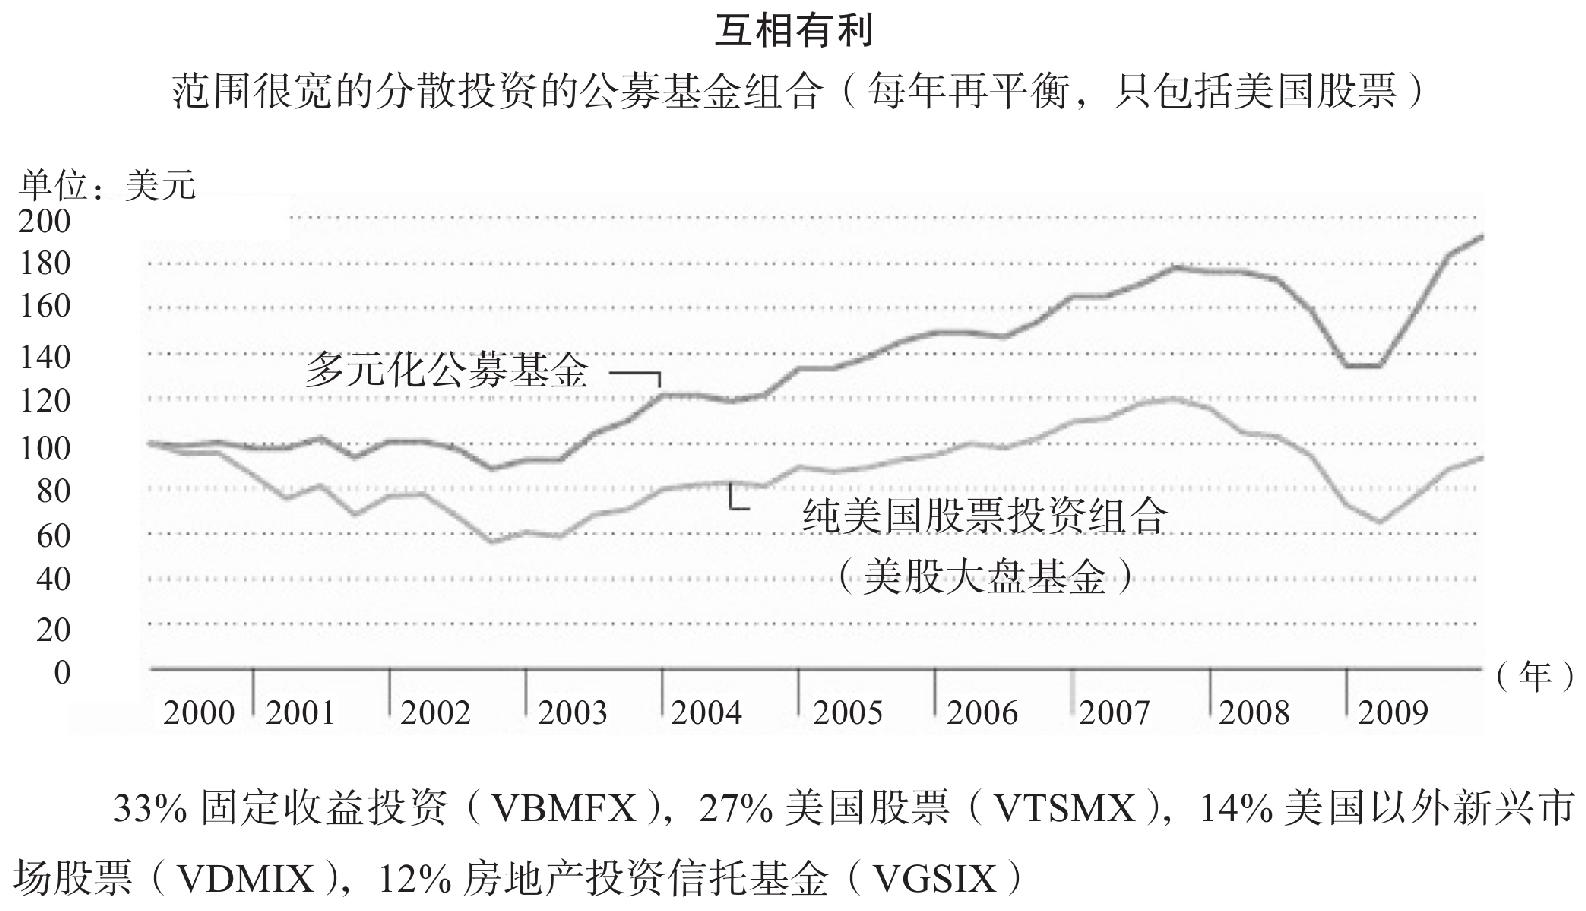
\includegraphics[width=0.96\linewidth,keepaspectratio]{image/25-3.jpg}
\caption{}\label{fig:25-3}
\par\smallskip{\footnotesize 数据来源：先锋公司和晨星公司\par}
\end{figure}

第2个指数，它持续稳定上涨5年，你5年累计投入5000美元本金，变成5915美元，收益率为18.3\%，这也不错。

但是在一个波动的市场，你的本金还是5年累计投入5000美元，最终增值到6048美元，收益率是20.96\%。二者相比，波动性强的市场比稳定增长的市场给你带来的利润率相对要高出2.66\%！伯顿·麦基尔告诉我，问题是大多数人不愿意利用波动性强的市场走势来让自己多赚钱。市场一下跌，他们就受不了了，马上大叫：‘我的天哪！跌了这么多，我得赶紧卖掉！’所以你必须保持头脑清醒，继续按照计划稳定地定期买入，这样才能赚到更多的钱。

2000—2009年，投资者学到了痛苦的教训，我们知道，从股市周期来看，这是失落的10年。如果你把钱放到美国股市上，从2000年年初开始到2009年年底结束，你就会很惨。投资标准普尔500指数，1999年12月31日投资1美元，到了2009年年底只有0.9美元，投资10年，你还亏了10\%，真是失落的10年。根据伯顿·麦基尔的计算，同样是这失落的10年，如果你用基金定投定期定额分散时间投入，你不但不会亏，而且能赚到不少钱。

伯顿·麦基尔给《华尔街日报》写了篇文章，标题是《“买入并一直持有”才是赢家》。在文中他解释道，自己支持买入并长期持有的事实依据是，如果你分散投资到一些指数基金组成的篮子里，包括美国股票、外国股票、新兴市场股票、房地产，从2000年年初到2009年年底，初始投入资本为10万美元，10年后增长到191859美元，这10年累计收益率为91.9\%，年化收益率是6.7\%。同样是在这个失落的10年，标准普尔500指数不但没有上涨，而且下跌了10\%。

“基金定投能让市场波动为你所用，替你赚更多的钱。”伯顿·麦基尔告诉我。

从巴菲特的导师本杰明·格雷厄姆到伯顿·麦基尔，再到很多受尊敬的学术专家，每个人都有一个理由支持你运用基金定投，从你持续稳定的收入中，定期拿出来一个固定的百分比定额买入，做到在时间上分散投资。但是如果你有很大一笔资金要做投资，那么基金定投不是最好的办法。如果你现在属于这种情况，那么看一下下面的内容。

基金定投即定期定额投资，意思是有系统地、按部就班地每次投入同样数量的资金。但这是从整个投资组合来说的，而不只是股票那一部分。

记住，要让波动市场成为你的朋友，你要使用基金定投，同时还要考虑使用另外一种投资技巧，让自己一直保持在正常的轨道上，这就是“再平衡”。

那么，让基金定投为你有效地工作的最好的办法是什么？幸运的是，大多数人都有401(k)账户或者403（b）账户\footnote{\label{fn:pdf-25-2}403（b），美国教育机构或者非营利组织雇员的退休金计划。——编者注}，可以按照一个固定的时间表，每次自动地投资相同的金额，这其实就是基金定投，让你享受到基金定投带来的好处。但是如果你没有这样一个自动化操作的基金定投系统，也没关系，你很容易就能设置一个。我有一个搞个体经营的朋友，她在先锋公司设置了一个退休投资账户，并享有税收优惠。她授权先锋公司每个月从她的银行账户自动扣款1000美元，投资她指定的多家指数基金，它们类型不同，而且相当分散。她知道自己并不能约束自己按照计划买入，特别是她感觉市场涨得太高时自己可能嫌贵不愿意买入，或者她感觉市场跌得太低时自己又可能因为恐惧而不敢买入，所以她干脆让自己置身事外。她是一个长期投资者，做了基金定投之后，就再也不用担心择时的问题了，因为她的操作体系已经自动化了，买入决策权根本不在她的手中。

有种方法能让你做基金定投更加容易，就是你到堡垒投资理财顾问公司开个投资账户，这家公司会帮你自动做基金定投。

你还要记住，在下面，我会向你展示一个非凡的投资工具，它能保护你在市场波动的时候避免损失。用了这个工具，即使你的市场择时完全错得离谱，你在股市上也不会损失一分钱。但是如果你的市场择时做对了，你会赢更多。但是在此之前，我们来看看第二个久经考验的投资模式，它能够保护你的积蓄，帮助你的财务自由基金增值最大化，为你增加更多的财富。

\subsection{避免的模式：要做再平衡}

戴维·斯文森和伯顿·麦基尔有时会采取不同的投资理财方法。但是有一点他们俩都跟我说过，所有我采访过的其他专家也都一致赞同这一点：要成为一个成功的投资者，你必须把投资组合定期再平衡。

你需要看看你的两个水桶，确认你的资产配置仍然是合适的比例。隔一段时间，你的水桶里的某一部分投资也许会大幅增长，与你投资组合里的其他部分一比，资产配置比例明显不合适，这让你的资产配置失去了平衡。

比如，你一开始的大类资产配置比例是6∶4，60\%的钱放在风险/成长水桶，40\%的钱放在安全/安心水桶。过了6个月，你检查你的投资账户发现，现在你的风险/成长水桶里面的投资大涨了，结果导致风险/成长水桶里面的资产占整个组合总资产的比例不是60\%，而是75\%了，那你现在的安全/安心水桶占总资产的比例只有25\%，而不是原来的40\%。原来两大水桶的大类资产配置比例是6∶4，现在成75∶25，明显偏离你设定的目标资产配置比例，所以现在你需要再平衡！

就像定期定额投资一样，再平衡也是一项技术。它乍一看很简单，但是真的要做到需要很多的规则，除非你牢牢记住再平衡非常重要，能让你的利润最大化，保护你免受亏损，而且它非常有效。否则，你会发现追涨杀跌的动量交易会迷住你，让你觉得现在自己短线投资的成功将会永远持续下去，或者现在的市场（股票市场、房地产市场、债券市场、商品期货市场）只会沿着一个方向继续前进：上涨，上涨，再上涨。

这种情绪和心理模式导致了人们持有一种投资时间过长，结果他们把原来引以为傲的巨大收益又还给了市场，这就像坐了一次过山车。遵守规则，你才会在某项投资还在继续上涨的时候，敢于逆市卖出，也让你能够在某项投资正在下跌时，或者在横盘上涨非常缓慢的时候，勇于逆势买入。

实践这个逆向投资的原则有一个非常有说服力的案例，那是一个真实的案例——投资界的偶像人物卡尔·伊坎在网飞公司（Netflix）股票上的投资操作。有一天，我去拜访他，正好刚有新闻报道说他投资Netflix股票赚了接近8亿美元。这部分股票都是他在一年之前，在每股58美元的时候买入的，现在的市场行情价格是每股341美元。他的儿子布雷特和他一起工作。最初这只股票的投资机会是他儿子给他的，他儿子不同意卖出这只股票，因为他觉得这只股票将来还有很大的增长空间。卡尔·伊坎说，他同意这个看法，但是他们的投资组合需要再平衡。如果他们不做再平衡的话，他们会发现自己可能会损失一些已经到手的巨大收益。卡尔在Netflix股票上一年赚了487\%，带着这笔巨大的盈利，他投资了组合里的其他资产，同时他手上还保留了2\%的Netflix股票，继续享受这只股票的未来增长。他用其中一部分资金购买了一家小公司的股票，公司名字是“苹果”（当时来看）。他认为当时这只股票被过于低估了。他高位卖出，低位买入，这就是投资的最高境界。再平衡是这个过程的核心。

\subsection{如果亿万富翁这么做，也许你也应该这么做}

你如果发现投资组合失去平衡了，应该怎么做？你原来的大类资产配置比例是6∶4，60\%的资产配置在风险/成长水桶，40\%的资产配置在安全/安心水桶。但是就我前面所描述的那样，你的股票猛涨，结果变成了75∶25，在这种情况下，你的再平衡行动计划要求你进行再平衡，把一些原来按照计划准备增加到风险/成长水桶的资金，转移到这个安全/安心水桶中，加快安全/安心水桶的资产增加速度，直到其在总资产中所占的比例重新回升到40\%。另一种做法是，你可以把一部分风险/成长水桶里涨了很多的投资，趁着行情很火，高位卖出，然后把拿回来的资金用来增加安全/安心水桶里面的投资，比如投资债券或者第一信托契约或者其他的资产。但是这样再平衡的过程可能会很痛苦，特别是，房地产投资信托基金正在猛涨，或者国际股票突然一下子上升，放着嘴里的肥肉不吃，转身离去，真的很痛苦。当乘坐一枚火箭飞速上升时，谁愿意跳下来？你只想要股票涨得更高！但是就像在赌场赌钱一样，手风大顺，赢了很多钱，现在是时候把桌子上赢的钱拿走一部分，以减少你的风险暴露程度了。同样的道理，你必须把你一部分涨得很猛的资产减持一些，以确定你在账面上赚的钱真正地赚到了手里，赚到手里的钱才是真正的钱。

就像定期定额投资一样，你必须抽离情绪，置身事外。投资组合再平衡，让你做的事和你想做的事正好相反，在投资中，这往往才是你应该去做的正确的事。

我们来看一个真实的案例：2013年夏，标准普尔500指数正在持续上涨，创出了历史新高，而这时的债券市场低迷，只能勉强产生少得可怜的收益率，你会卖出股票，买入债券吗？不可能！但是再平衡的法则就是这么说的，这正是你需要做的，卖出一部分大涨的股票，买入一部分低迷的债券，以保持你原始的资产配置比例——即使你内心有个声音在狂喊：“嘿，蠢货，为什么你要卖出股票拿钱去买那些债券？”

再平衡法则并不能保证你每次都能赢，但是再平衡意味着你赢的次数更多一些。再平衡增加了你获得成功的机会。经年累月，机会才是决定你的长期投资生涯成功还是失败的关键因素。

资深投资者总是会在不同的市场之间、不同的资产类型之间进行再平衡，当然这样做可能会使人感到更加痛苦。

比如，你有很多苹果公司的股票，正是在2012年7月，当时你要是卖出这些股票看起来简直就是脑子不正常，因为它们一直在猛涨——只前两个季度就涨了44\%，现在股价超过每股614美元。但是如果苹果公司的股票在你的投资组合里占了很大的资产比例（记住，苹果公司股票刚刚上涨了44\%，让你的投资组合失去了平衡，失衡程度应该相当大），再平衡法则告诉你必须卖掉一些苹果公司的股票，让你的资产配置比例重新回归合理的配置水平。卖掉正在上涨的大牛股，简直是要了你的命！但是再过一年后，同样是7月这个时间，你会不会感谢自己？为什么？苹果公司的股票行情走势像过山车一样，从2012年9月最高的705美元，跌到2013年年初最低的385美元，到2013年7月其收盘价为414美元——做了再平衡，让你避免了41\%的损失。

那么应该多久进行一次再平衡？大多数投资者可以每年一次或者每年两次进行再平衡。玛丽·卡拉汉·厄道斯告诉我，她非常相信再平衡是强大的工具，所以她“经常”进行再平衡。“经常”意味着多久？“对比你原来合理设置好的各部分资产类型的资产配置比例，经常检查你的投资组合，只要发现明显偏离了目标配置比例，你就要进行再平衡。多少次出现明显不一致，你就要相应地进行多少次再平衡，调整你的资产配置比例，改变你的投资计划，以适应世界上发生的新情况。你应该经常重新评估，但是不要过分密集地重新评估。”

另一方面，伯顿·麦基尔喜欢充分利用牛市上涨的势头。他建议资产平衡只要一年做一次就够了。我不想当个好战派，只是因为一个投资上涨了就要卖掉，理由是马上再平衡。”他说，“我希望给我市场表现好的资产类型至少一年的时间，让子弹再飞一会儿。”

不管你多久做一次再平衡，记住，它不但可以保护你避免承担过多的风险，而且可以大幅增加你的投资收益，就像定期定额投资一样。正是规则再次让你投资市场表现差的资产，这个时候的买入价格更低，所以你用同样的投资额可以购买更多的资产，所以等到价格上涨的时候，你手上持有的这种资产类型的数量就更多，赚的自然也更多。在这个过程中，你的利润是你的团队里面其他选手传给你的，就像洛杉矶湖人队进攻时球在不停地转移，或者就像接力赛跑的选手一样，一棒接一棒地不断交接，最终你会胜利到达终点。

你做再平衡的次数确实对你的税收有影响。如果你的投资不是在一个可以递延纳税的环境下，再平衡一项持有不到一年的资产，卖出一部分或者全部，一般要交税率更高的个人收入所得税，而不是税率更低的长期投资税。

再平衡，听起来或许让你有点儿害怕，好消息是这个工作也可以自动化，堡垒投资理财公司或者你选择的其他受托人投资顾问都可以帮你做到。投资顾问会指导你既提高你的税收效率，又继续发挥再平衡的力量。

现在你已经学到了两个久经考验的投资应用，以减少你的风险，增加你的收益。你不需要做别的，只要做资产配置就行了。但是还有最后一个技巧可以让你去掉两个“肉中刺”——亏损和税收。

\subsection{收获的时候到了}

组合再平衡的时间到了，你必须卖出一部分股票，这些股票不属于你的401(k)账户或者其他有税收优惠的账户，那么这会发生什么情况？美国政府会伸出税收之手，只要是你赚的钱，它都要抽走一部分作为税收。是不是资本利得税会让你痛苦得发疯？听着，这里有一个完全合法的办法让你可以降低税款，同时让你的投资组合继续保持平衡，这就是税收损失收割法。税收损失收割法的好处是减少你的税收，增加你的净收益。从本质上讲，你用自己一些不可避免的亏损来最大化你的税后净收益。

伯顿·麦基尔认为，税收损失收割法可以增加你的年收益率，每年增加的比例高达1\%，所以这值得你好好研究一番。

亿万富豪和大型机构都用这种方法来增加他们的投资收益率，但是普通投资者很少会利用这个强大、有效的技术，很少有人知道，即使那些知道的人也会觉得，这个再平衡和税收损失收割法听起来太复杂了，不愿意自己亲身尝试一下。不要担心，你可以询问受托人投资顾问或者用软件来做，就像在网上订购一份比萨一样，或者至少可以说，难度就像更新你的推特的安全设置一样，没你想象的那么复杂。

现在，请牢记在心，我的目标是让投资变得更简单，每个人都能做到，这个部分是本书技术含量最高的，最能考验你的大脑！首先祝贺你一直紧紧地跟着我学习完成最难的一部分。这部分的内容会让你感觉很有技术含量，大多数人会像躲避瘟疫一样远远地躲开。资产配置，基金定投，再平衡，税收损失收割法，这些术语一听就让你头疼，我希望你能知道，所有这些东西都可以设置成自动化操作，不用你自己动手操作。但是，清楚理解这些策略的意义，以及这些策略有效的主要原因，对你还是很有帮助的。

在本书第四部分，你只需要牢记4件事就够了。

第一，配置决定一切！所以你要进行大类资产配置，把它们分散投资到两大水桶中：安全/安心水桶和风险/成长水桶。做到分散投资到不同的资产类型、不同的市场、不同的时间。

第二，你不用犹豫不决，因为你想找到完美的入市时机。相反，你要利用定期定额投资，你知道波动会成为你的朋友，市场下跌会提供给你便宜买入的机会。当市场重新反弹回来的时候，这项投资技术会增加你投资组合的整体价值。

第三，要有一个梦想水桶，给你提供情绪上的快乐和兴奋。所以你可以体验到你的勇敢投资在短期和中期所带来的好处，而不是要等到遥远的未来才能享受到。

第四，用税收损失收割法把你的收益最大化，把你的损失最小化。

我第一次提出，我要在本书里讲资产配置以及基金定投等这些相关的精妙策略时，我的金融圈里的很多朋友都说：“你疯啦？这些东西太复杂了，一般人根本搞不懂，很少有人愿意花时间读这些复杂难懂的东西。”我的回答很简单：“我在这里写书，是要写给那些少数行动派而不是多数空谈派的。”你需要饥饿感才能推动自己去掌握一些新东西，但是在掌握投资基本原则这件事上，你下的功夫绝对会有超值回报的。即使你必须来来回回地读上两三遍才能弄明白其中的道理，但你弄懂了之后的回报会非常大、非常多、非常久——这意味着会节省你好多年辛辛苦苦工作的时间。更重要的是，掌握了这些会给你一种感觉：上天赋予我更多的权力，我的内心更加安宁。

掌握资产配置这一部分很像第一次学习开一辆手动挡的汽车。开这样的车，我要一边使用加速器、刹车、离合器、变速杆、后视镜、方向盘，一边还要看着路面。你开玩笑吗？但是过段时间你就能开着车飞奔了，想都不用想这些问题了。

好了，我们现在一起走了很长一段路，在7步通向财务自由之路上走完了前四步。让我们回头看一下我们走过的路。

第一步，你做了一生最重要的投资理财决策，决定从你的收入中拿出一定的比例储蓄起来，作为财务自由基金，自动进行投资获取复利。你是不是已经做好这一步了？只要开个银行自动扣款的账户就行了。如果没有，今天就去做！

第二步，你学到了投资的门道，也知道了如何避免证券市场9个最大的投资误区，其实就是投资营销谎言。你成了下棋的棋手，而不是被棋手摆弄的棋子。

第三步，你已经走过了7步通向财务自由之路的第三步，让投资游戏能赢。这一步分为三个阶段：第一阶段，你计算出来你的三个地位最重要的财务目标，对于很多人来说它们是财务安全、财务活力、财务独立。第二阶段，你有了一个投资理财计划，计划的目标数字不是拍脑袋随便想出来的，而是根据实际情况推算出来的实实在在的数据。第三阶段，你寻找并实施一些方法来加快你的计划进展速度，这样你可以更早地享受你的投资回报。

第四步，你做出了一生最重要的投资决策，就是把你的资产配置到一个投资组合。每个水桶都有一个具体明确的资产配置比例（安全/安心水桶、风险/成长水桶、梦想水桶）。你已经做了充分的分散投资，并有了一个计划，它能加速实现你的财务梦想。

现在你在投资理财上已经甩开了99\%的美国人，甚至是全世界其余99\%的投资人，你对投资的理解深度，对投资管理实务的理解深度，都明显像个内行了。有些人对我很好，花了很多时间读了本书的初稿，他们有一个相同之处，那就是在学到这些东西之后，他们心里非常激动。如果你和他们一样，你就会跳上跳下，抓住你的朋友的肩膀，想展示给他们你刚刚学到的一些投资理财方法，因为这样做能给他们增加几十万美元，甚至是几百万美元的投资收益。但是你也许会吃惊地发现，自己让朋友泼了一头冷水：你一分钱还没有见着呢！我向你保证，最好的东西还在后面。从现在开始，后面的内容会比这个部分容易得多。

现在，既然你所想所做的都像一个投资内行一样，我会展示给你看，如何真正像内行一样去投资。让我们来看一看，你如何能在任何金融环境下都取得成功，你如何能够获得市场上行的潜在收益而不用承担市场下行的风险，创造出一个终身收入流。

\subsection{定期定额投资与一次性大额投资比较}

如果你有大笔钱要去投资，定期定额投资对于你来说是最好的方法吗？

如果你突然发了大财，比如得到10000美元奖金，就像我们在这个部分前面所说的那样，或者你得到了5万美元的保险赔付金，那么你是用基金定投，按照固定的时间表，分成几个月甚至几年，分期分批每次买入固定的金额，还是干脆一次性做大笔投资呢？

这里就有矛盾和争议了。有些投资顾问反对基金定投，反对的理由也很客观，就连伯顿·麦基尔也承认要投资股市，如果股市一直上涨的话，基金定投并不是最高效的策略，就像美国经济大萧条之后的几年，美国股市就一直在上涨。

要是在牛市的一开始，你就把所有资金一次性全部投入，肯定比把它分成60小份，用5年时间每个月做基金定投赚的钱更多。这很明显，对不对？最近有些研究表明，其中包括先锋公司在2012年做的研究，按照10年为一期滚动计算，在过去80年里，在美国、英国、澳大利亚三个股票市场里，一次性大额投资在超过2/3的时间里，都胜过基金定投。

为什么会是这样？因为一次性大额投资，你投进去的钱更多，资金开始替你赚钱的时间更早，而且从长期来看，交易次数少，可以把交易费用控制得更低。一次性大额投资，在牛市里，肯定能给你带来获得更大潜在收益的机会，但是如果市场下跌，它也会给你带来更大的整体亏损。研究表明，长期而言，一次性大额投资，如果在分散投资上做得好的话，你会赚更多的钱。你能多赚多少钱？最终，平均而言你最多能够增加2.3\%的收益率。还记得伯顿·麦基尔计算出来的基金定投效果的实际数据吗？在2000—2010年失落的10年期间，如果你投资1美元到标准普尔500指数，从1999年12月31日起10年之后，你只剩下0.90美元，投资10年亏损了10\%。但是如果你用的是基金定投，同样是这10年，你不但没有损失，而且会赚钱。在这些研究中，有些研究说一次性大额投资好，有些研究说基金定投好，那么你到底该怎么做？你得到10000美元奖金，会马上全部投入股市，还是会先把这10000美元放在一个更加安全的地方，然后做基金定投，用10个月时间，你每个月投资1000美元呢？如果是前面说的一次性拿到了5万美元保险赔付金，用2年的时间来做基金定投，如果市场持续上涨，你这样分期分批投入，要少赚不少钱。但是行为经济学告诉我们，你并不会为此感到后悔，相比之下，如果你一次性全部投入，结果2天之后股市崩盘了，你才会非常后悔！

所以这完全取决于你自己。我要再说一次，我到这里来不是来给你投资建议的，只是要分享给你全世界最优秀的投资理财专家的最高明的投资见解。对于大多数人来说，一次性大额投资并不是一个问题，因为他们手上根本没有这样一大笔钱！如果你正好没有这样一大笔钱，只能每个月靠工资攒点儿小钱，你仍然可以做基金定投，投资一个合理分散的投资组合，让自己的收益最大化，最终你也能赚到一笔大钱。
